\documentclass[11pt]{texMemo-gibbons}
\usepackage[english]{babel}
\usepackage{graphicx}
\usepackage{blindtext}
\usepackage{amsmath,amssymb,units}
\usepackage[outdir=./]{epstopdf}
\memostudent{Ty Davis}
\memocourse{ECE 3210}
\memosubject{Lab 1, Lab Basics}
\memodate{\today}
\logo{
\includegraphics[width=0.5\textwidth]{ece_horiz.pdf}}

\begin{document}
\maketitle

\section{Introduction}
\label{sec:introduction}

This is the first lab of the semester in which we cover
the lab basics. We will be doing a brief analysis of 
a circuit and then measuring and comparing the results of our
computation. 

\section{Theory}
\label{sec:theory}

The theory section of the memo should cover the theory
behind the lab.  For example, if there is a derivation
needed, include that here.  When you write up a derivation,
you don't need to show every single step of mathematical
manipulation, but you need to include enough steps such
that a typical engineer could follow it.  You must typeset
your equation using the \LaTeX  equation editor to make
it look good.

For example, suppose we need to compute the complex
exponential Fourier series coefficients for a saw-tooth
waveform.  We know that $T_0=2$ and $\omega_0=\pi$.
We write out the integral we need to solve

\begin{equation}
  \label{eq:1}
  D_n = \frac{1}{2}\int^2_0 t e^{-j\pi n t} dt.  
\end{equation}

We don't need to go through and show every step of the
derivation.  It would be sufficient to say that solving
the integral yields

\begin{equation}
  \label{eq:2}
  D_n = \frac{j}{\pi n}.
\end{equation}


\section{Results}
\label{sec:results}

The results section covers the results from the lab.
Your data will mostly be represented in plots and tables.
Include those figures AFTER the main body of text on
a new page.  Data interpretation (what the plots \emph{mean})
should be reserved for the Conclusions section of the
memo.  You should comment on the trends of what you
have seen, but do not explain \emph{why} you are seeing
them in this section.


\section{Discussion and Conclusions}
\label{sec:conclusions}

The conclusions section is for interpreting the data.
If you see a trend in your data, explain why you see
it in this section.  Use the theory you learned in class
in your explanation.

As a final note, you are expected to use this document
as a template for your lab submissions.  You are welcome
to upload this to overleaf to edit/compile the document.
Or you can work locally using whatever flavor of \LaTeX
compiler you prefer.  All you need to do is to upload
the document (and not the \LaTeX  source) to Canvas.

\clearpage

\begin{figure}[h!]
  \centering
  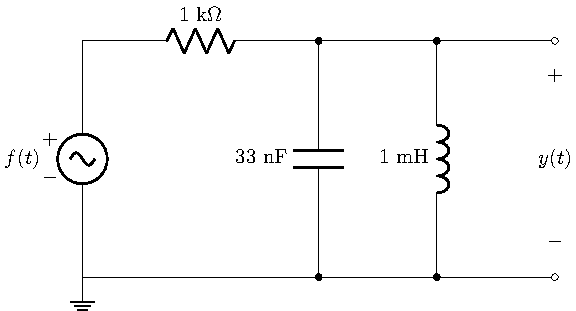
\includegraphics{circuits/circuit_01.pdf}
  \caption{Circuit for analysis in the main part of the lab.}
  \label{fig:plots01}
\end{figure}

\begin{figure}[h!]
  \centering
  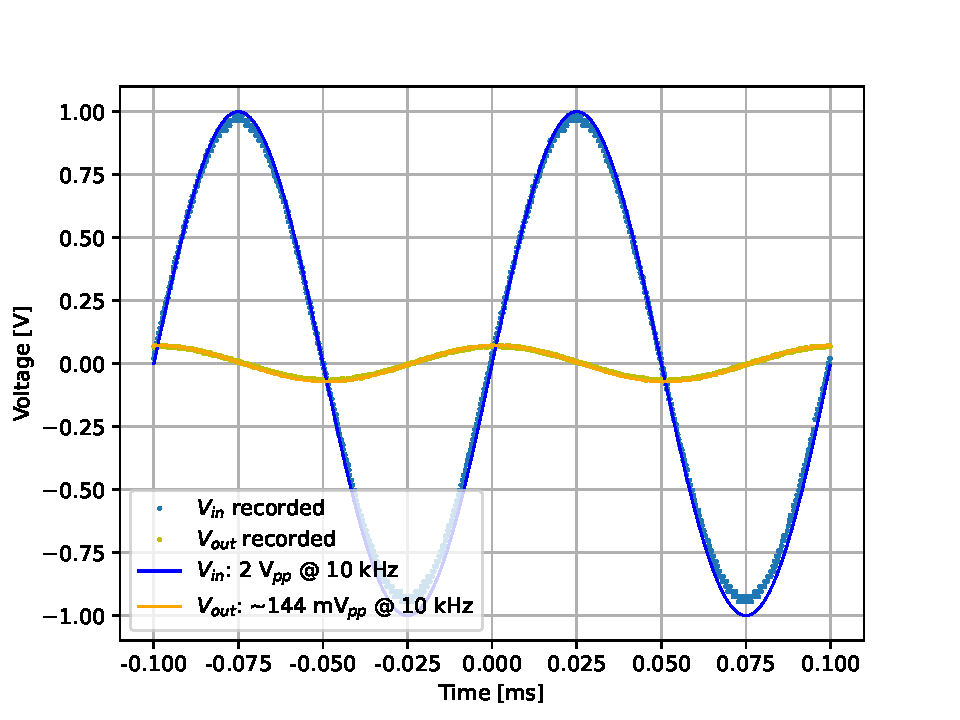
\includegraphics[width=0.7\textwidth]{plots/circuit_analysis.pdf}
  \caption{Plot for the circuit analyzed in Fig.~\ref{fig:plots01}}
\end{figure}

\begin{figure}[h!]
  \centering
  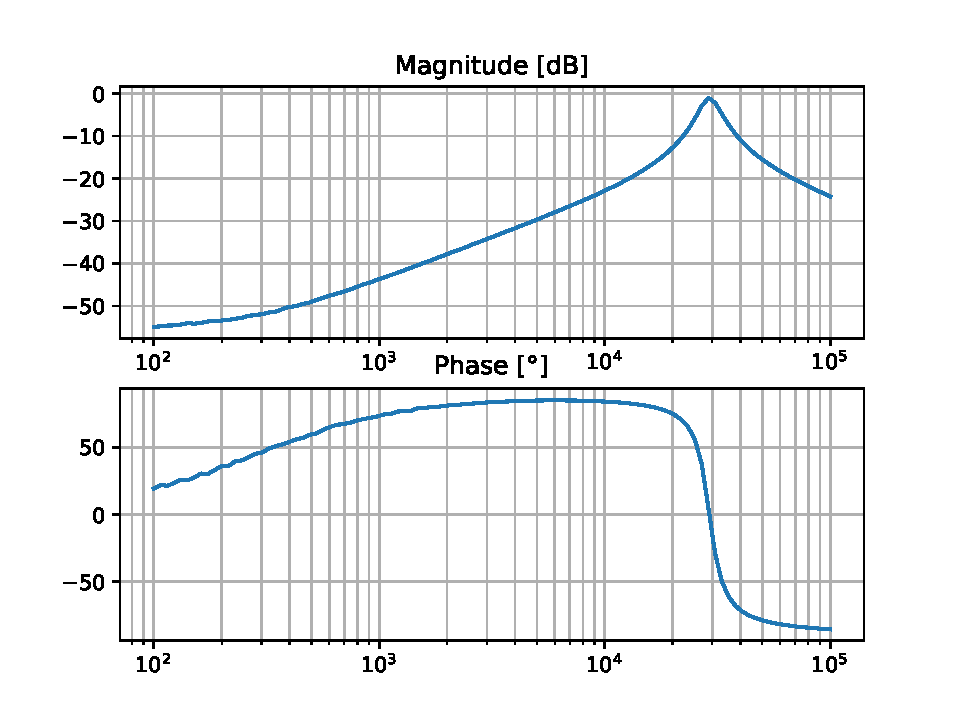
\includegraphics[width=0.7\textwidth]{plots/bode_plots.pdf}
  \caption{Bode plot of the frequency analysis for the circuit in Fig.~\ref{fig:plots01}}
\end{figure}


\end{document}
%%% Local Variables:
%%% mode: latex
%%% TeX-master: t
%%% End:
